\documentclass[11pt]{beamer}
\usetheme{Warsaw}
\mode<presentation>{}
\usepackage[utf8]{inputenc}
\usepackage[english]{babel}
\usepackage{amsmath}
\usepackage{amsfonts}
\usepackage{amssymb}
\usepackage{graphicx}
\usepackage{listings}
\usepackage{todonotes}
\usepackage{lmodern}
\author{Enrico Steffinlongo}
\title{Privilege separation in browser architectures}
\institute[Universities Here and There] % (optional)
{
  Università Ca' Foscari - Computer science
}
%\date{}


%\setbeamercovered{transparent} 
\setbeamertemplate{navigation symbols}{} 
%\logo{} 
%\institute{} 
%\date{} 
%\subject{} 

\defbeamertemplate*{footline}{shadow theme}
{%
  \leavevmode%
  \hbox{\begin{beamercolorbox}[wd=.5\paperwidth,ht=2.5ex,dp=1.125ex,leftskip=.3cm plus1fil,rightskip=.3cm]{author in head/foot}%
    \hfill\insertshortauthor
  \end{beamercolorbox}%
  \begin{beamercolorbox}[wd=.5\paperwidth,ht=2.5ex,dp=1.125ex,leftskip=.3cm,rightskip=.3cm plus1fil]{title in head/foot}%
    \usebeamerfont{title in head/foot}\insertshorttitle\hfill\insertframenumber\,/\,\inserttotalframenumber%
  \end{beamercolorbox}}%
  \vskip0pt%
}

% basics
\newcommand{\names}{\mathcal{N}}
\newcommand{\vars}{\mathcal{V}}
\newcommand{\perms}{\mathcal{P}}
\newcommand{\refs}{\mathcal{R}}
\newcommand{\caller}{\mathbf{caller}}

\renewcommand{\vec}[1]{\overrightarrow{#1}}
\newcommand{\subst}[2]{[#1/#2]}
\newcommand{\overwrite}[2]{[#1 \mapsto #2]}
\newcommand{\xra}[1]{\xrightarrow{#1}}
\newcommand{\xRa}[1]{\xRightarrow{#1}}
\newcommand{\hra}{\hookrightarrow}
\newcommand{\fv}{\mathit{fv}}
\newcommand{\fn}{\mathit{fn}}
\newcommand{\fnfv}{\mathit{fnfv}}
\newcommand{\map}[3]{#1 \stackrel{#2}{\mapsto} #3}
\newcommand{\dom}{\mathit{dom}}
\newcommand{\defined}[1]{#1\!\downarrow\ }

\newcommand{\powerset}[1]{2^{#1}}
\newcommand{\jm}{\mathcal{J}}
\newcommand{\fvbv}{\mathit{vars}}

\newenvironment{mcases}[0]{\begin{list}{{\em Case}}{\leftmargin 5pt}}{\end{list}}

% permission
\newcommand{\join}{\sqcup}
\newcommand{\meet}{\sqcap}
\newcommand{\compl}[1]{#1^*}

% values
\newcommand{\lam}[2]{\lambda #1.#2}
\newcommand{\rec}[1]{\{#1\}}
\newcommand{\unit}{\mathbf{unit}}
\newcommand{\true}{\mathbf{true}}
\newcommand{\false}{\mathbf{false}}
\newcommand{\str}[1]{``\mathit{#1}''}
\newcommand{\undef}{\mathbf{undefined}}

% expressions
\newcommand{\letexpr}[3]{\mathbf{let}\ #1 = #2\ \mathbf{in}\ #3}
\newcommand{\appl}[2]{#1\, #2}
\newcommand{\op}{\mathit{op}}
\newcommand{\cond}[3]{\mathbf{if}\ (#1)\ \{\ #2\ \}\ \mathbf{else}\ \{\ #3\ \}}
\newcommand{\while}[2]{\mathbf{while}\ (#1)\ \{\ #2\ \}}
\newcommand{\lookup}[2]{#1[#2]}
\newcommand{\store}[3]{#1[#2] = #3}
\newcommand{\delete}[2]{\mathbf{delete}\ #1[#2]}
\newcommand{\err}{\mathbf{err}}
\newcommand{\newref}[2]{\mathbf{ref}_{#1}\ #2}
\newcommand{\deref}[1]{\mathbf{deref}\ #1}
\newcommand{\setref}[2]{#1 = #2}
\newcommand{\send}[3]{\overline{#1} \langle #2 \triangleright #3 \rangle}
\newcommand{\checkperms}[2]{\mathbf{check}(#1,#2)}
\newcommand{\acquire}[1]{\mathbf{acquire}(#1)}
\newcommand{\release}[1]{\mathbf{release}(#1)}
\newcommand{\register}[3]{\mathbf{register}(#1,#2,#3)}
\newcommand{\exercise}[1]{\mathbf{exercise}(#1)}
\newcommand{\self}{\mathbf{self}}

\newcommand{\match}[2]{\mathbf{match}\ #1\ \mathbf{with}\ \{#2\}}
\newcommand{\checkp}[3]{\mathbf{check}(#1)\ \mathbf{then}\ #2\ \mathbf{else}\ #3}

% components, systems and states
\newcommand{\handler}[5]{#1(#2 \triangleleft #3:#5).#4}
\newcommand{\inst}[3]{#1\{\!|#2|\!\}_{#3}}
\newcommand{\para}[2]{#1 \parallel #2}
\newcommand{\sys}[3]{#1;#2;#3}

\newcommand{\ctx}[2]{#1\langle #2\rangle}
\newcommand{\labcall}[4]{\langle #1:#2,#3:#4 \rangle}
\newcommand{\labex}[3]{#1:#2 \gg #3}

% misc
\newcommand{\lambdaJS}{\lambda_{\mathsf{JS}}}
\newcommand{\irule}[1]{({\sc #1})}

% flow logic
\newcommand{\labs}{{\mathcal L}}
\newcommand{\absenv}{\hat{\Gamma}}
\newcommand{\absflow}{\hat{\phi}}
\newcommand{\absnet}{\hat{\Phi}}
\newcommand{\absvalues}{\hat{V}}
\newcommand{\absmem}{\hat{\mu}}
\newcommand{\abscache}{\hat{\Phi}}
\newcommand{\absassert}{\hat{L}}
\newcommand{\forms}{\Phi}
\newcommand{\terms}{\mathcal{T}}

\newcommand{\absop}{\widehat{\op}}
\newcommand{\abseq}{\widehat{eq}}
\newcommand{\absget}{\widehat{get}}
\newcommand{\absset}{\widehat{set}}
\newcommand{\absdel}{\widehat{del}}

\newcommand{\dontcare}{\diamond}
\newcommand{\abscaller}{\widehat{\caller}}
\newcommand{\msg}{\mathbb{M}}
\newcommand{\abself}{\widehat{\self}}
\newcommand{\absform}[1]{\langle #1 \rangle}
\newcommand{\hasperm}[2]{#1\ \mathsf{has}\ #2}
\newcommand{\ltrue}{\mathsf{true}}
\newcommand{\lacquire}[3]{#1 \uparrow #2,#3}
\newcommand{\lrelease}[3]{#1 \downarrow #2,#3}
\newcommand{\abstrue}{\true}
\newcommand{\absfalse}{\false}
\newcommand{\absunit}{\unit}
\newcommand{\absundef}{\undef}
\newcommand{\absrec}[1]{\langle\!| #1 |\!\rangle}
\newcommand{\abslam}[2]{\lambda #1^{#2}}
\newcommand{\absfuns}{\Lambda}

\newcommand{\absC}{{\cal C}}

% debundling
\newcommand{\avail}[1]{\mathit{Avail}_{#1}}
\newcommand{\req}[1]{\mathit{Req}_{#1}}
\newcommand{\psubst}[3]{[#1/#2]@#3}
\newcommand{\unbundle}[3]{#1 \rhd_{#2}\, #3}
\newcommand{\absE}{{\cal E}}
\newcommand{\rewrite}[1]{\succ #1}

% escalation
\newcommand{\abstack}{\hat{\Upsilon}}
\newcommand{\escalate}[1]{\,\gg #1}
\newcommand{\despite}[1]{\ \mathbf{despite}\ #1}
\newcommand{\permsleak}[1]{\mathit{Leak}_{#1}}

%other mine
\newcommand{\vat}[0]{\hat{v}}
\newcommand{\ljs}{$\lambda_{JS}$}

\begin{document}

\begin{frame}
\titlepage
\end{frame}

%\begin{frame}
%\listoftodos
%\end{frame}

\begin{frame}
\tableofcontents
\end{frame}

\section{Intro}
%\subsection{Browser extensions}
\begin{frame}{Browser Extensions}
Web browsers extensions are phenomenally popular.
\begin{itemize}
\item roughly 33\% of Firefox users have at least one add-on
\end{itemize}
Extension customize the user experience
\begin{itemize}
\item Customize the user interface
\item Adds lots of functionality to the browser (e.g., save and restore tabs)
\item Protect users from certain contents of the web pages 
\end{itemize}
\end{frame}

\begin{frame}{Browser Extensions}
Extension need to interact with
\begin{itemize}
\item Web pages DOM
\item Browser internal structure (tabs collections, \dots)
\item Browser API (browser storage, cookie jar, \dots)
\end{itemize}
Potential security problem!
\begin{itemize}
\item Browser API $\Rightarrow$ security critical operations\\
\item Web interaction $\Rightarrow$ Untrusted and potentially malicious\\
\end{itemize}
\end{frame}

\subsection{Chrome Extension}
\begin{frame}{Chrome extensions architecture}
A chrome extension is composed by
\begin{itemize}
\item A manifest: the file containing all 
\item A set of Content scripts
\item An Extension Core (composed by a set of scripts)
\item Other resources
\end{itemize}
\end{frame}

\begin{frame}{Chrome extensions architecture}
\begin{columns}[T]
\begin{column}{.48\textwidth}
Chrome extension architecture force developers to three practices
\begin{enumerate}
\item Privilege separation
\item Least privilege
\item Strong isolation
\end{enumerate}
\end{column}%
\begin{column}{.48\textwidth}
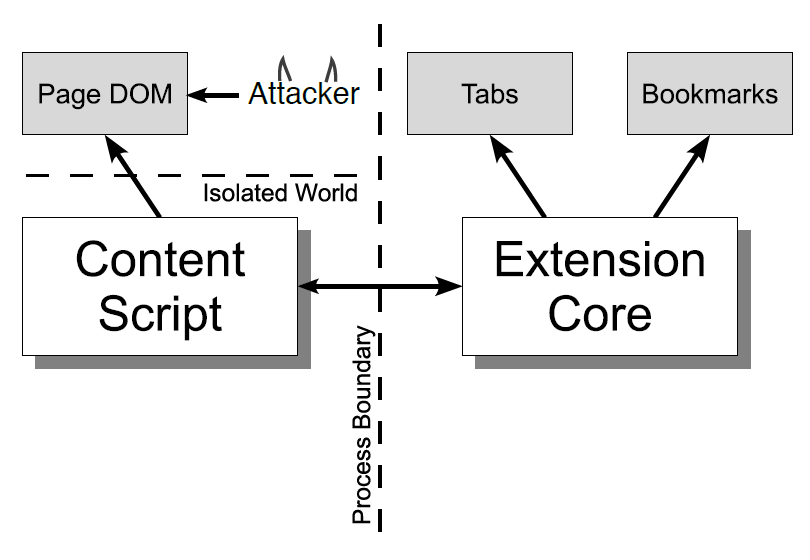
\includegraphics[scale=0.25]{Images/StrongIsolation.png}
\end{column}%
\end{columns}
\end{frame}

\begin{frame}{Privilege separation}
\begin{itemize}
\item Content scripts
\begin{itemize}
\item Injected to each page (multiple instances)
\item Access the DOM of the page
\item Cannot use privileges other than the one used to send messages to the Extension Core
\end{itemize}
\item Extension Core
\begin{itemize}
\item Single instance for each browser session
\item No access to DOM of pages
\item Can use privileges defined statically in the manifest
\end{itemize}
\end{itemize}
\end{frame}

\begin{frame}{Least privilege}
An extension has a limited set of permission defined statically in the manifest
\begin{itemize}
\item An extension cannot use more than required permissions
\item User have to agree with the required permission at install time
\item Attacker cannot use more than such set of privileges
\end{itemize}
\end{frame}

\begin{frame}{Strong isolation}
\begin{itemize}
\item Extension core is sandboxed in a process separated from the content scripts with unique origin
\item Communication between Extension Core and Content Scripts is only via message passing
\item Messages exchanged can only be string (Objects are marshaled using a JSON serializer without functions)
\item Content script are executed in a isolated world from web pages
\end{itemize}
\end{frame}

\begin{frame}{Isolated worlds}
\begin{columns}[T]
\begin{column}{.62\textwidth}
\begin{itemize}
\item Content script and web pages has different memory spaces
\item Only standard DOM fields are shared
\end{itemize}
A potentially malign web page cannot:
\begin{itemize}
\item alter the content of variables of the content script
\item invoke or share function with the content script
\end{itemize}
\end{column}%
\begin{column}{.33\textwidth}
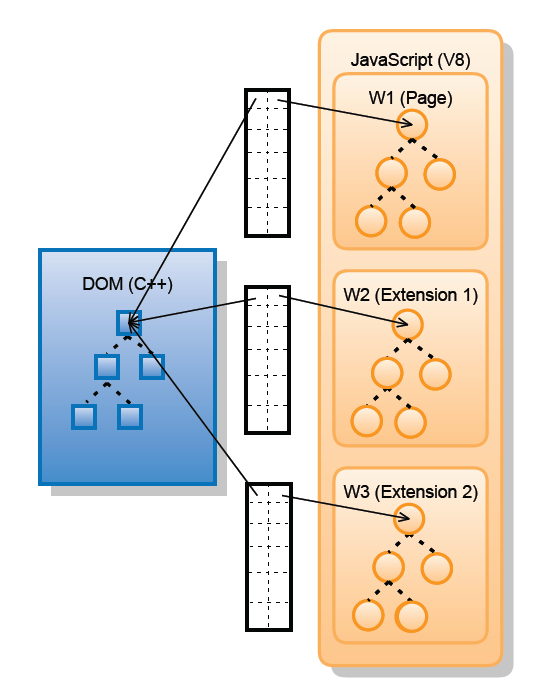
\includegraphics[scale=0.28]{Images/IsolatedWorlds.png}
\end{column}%
\end{columns}
\end{frame}

\begin{frame}{Message passing}
\todo[inline]{to be fixed MPI}
Chrome extension message passing API
\end{frame}

\begin{frame}{Bundling}
Extensions are often made by developer that are not security experts.
\todo[inline]{to be fixed Bundle}
Developer tends to manage incoming messages in a centralized way. This is dangerous because 

\end{frame}

\begin{frame}[fragile]{Example}
\todo[inline]{to be fixed Example}
\begin{columns}[T]
\begin{column}{.48\textwidth}

\end{column}
\begin{column}{.48\textwidth}
\begin{tiny}
\begin{lstlisting}
chrome.runtime.onMessage.addListener(
  function (msg, sender, sendResp) {
    if (msg.tag == "req") {
      var u = DB.getUser(msg.site);
      var p = DB.getPwd(msg.site);
      sendResp({"user": u, "pwd": p});
    }
    else if (msg.tag == "sync") {
      var db = DB.serialize();
      xmlhttp.open("GET", msg.site + db);
      xmlhttp.send();
    }
    else
      console.log ("Invalid message");
});
\end{lstlisting}
\end{tiny}
\end{column}
\end{columns}
\end{frame}

\section{Our work---}
\subsection{Analysis}
\begin{frame}{LambdaJS \cite{LambdaJS}}
\begin{columns}[T]
\begin{column}{.48\textwidth}
JavaScript:
\begin{itemize}
\item Complex language
\item Lots of constructs
\item unconventional semantics.
\end{itemize}
Very complex to analyze.
\end{column}
\begin{column}{.50\textwidth}
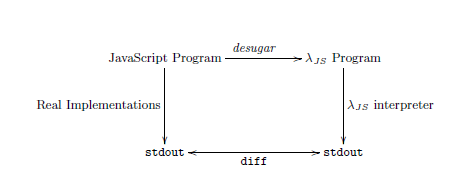
\includegraphics[scale=0.42]{Images/LambdaJS.PNG}
\end{column}
\end{columns}

\ljs\cite{LambdaJS} is a core calculus made by Brown university designed specifically to ``desugar'' JavaScript
\begin{itemize}
\item Few constructs
\item Standard $\lambda$-style semantics
\item Not a sound approximation of JavaScript
\item Tests on ``desugared'' files shows that its the semantic coincide with JavaScript
\end{itemize}
Easy to analyze
\end{frame}

\begin{frame}{The calculus}
\ljs++ is an extension of \ljs\ with security oriented constructs. Its components are:

\begin{itemize}
\item Constants: \begin{tiny}$c ::= \mathit{num} ~|~ \mathit{str} ~|~ \mathit{bool} ~|~ \unit ~|~ \undef$\end{tiny}
\item Values: \begin{tiny}$v ::= n ~|~ x ~|~ c ~|~ r_{\ell} ~|~ \lam{x}{e} ~|~ \rec{\vec{str_i:v_i}}$\end{tiny}
\item Expressions: \begin{tiny}$
\begin{array}{lcl}
e & ::= & v ~|~ \letexpr{x}{e}{e} ~|~ \appl{e}{e} ~|~ \op(\vec{e_i}) ~|~ \while{e}{e} \\
& | & \cond{e}{e}{e} ~|~  e;e ~|~ \lookup{e}{e} ~|~ \store{e}{e}{e} \\
& | & \delete{e}{e} ~|~ \newref{\ell}{e} ~|~ \deref{e} ~|~ \setref{e}{e} \\
& | & \send{e}{e}{\rho} ~|~ \exercise{\rho}.
\end{array}
$\end{tiny}
\item Memories: \begin{tiny}$\mu ::= \emptyset ~|~ \mu, \map{r_{\ell}}{\rho}{v}$\end{tiny}
\item Handlers: \begin{tiny}$h ::= \emptyset ~|~ h,\handler{a}{x}{\rho}{e}{\rho'}$\end{tiny}
\item Instances: \begin{tiny}$i ::= \emptyset ~|~ i,\inst{a}{e}{\rho}$\end{tiny}
\item System: \begin{tiny}$s = \sys{\mu}{h}{i}$\end{tiny}
\end{itemize}
\end{frame}

\begin{frame}{Judgments}
For the analysis we used Flow logic \cite{FlowLogic}
\end{frame}

\begin{frame}{Theorem}
Let $s = \mu;h;\emptyset$. If $\absC \Vdash s \despite \rho$, then $s$ is $\permsleak{\rho}(\absC)$-safe despite $\rho$.
\end{frame}

\subsection{Implementation}

\begin{frame}{Tool}
We developed a tool in F\# to perform the analysis described below. We:
\begin{enumerate}
\item add the chrome API definition as prelude to each source
\item desugar the source with prelude using the desugaring tool \cite{LambdaJS}
\item parse the desugared file using a YACC lexer/parser
\item alpha-rename all variables to avoid clashing since the analysis is context-insensitive
\item add unambiguous labels $\alpha$ on nodes in the AST ($e \Rightarrow e^\alpha$)
\item generate the constraints for the AST
\item solve the constraints using a worklist algorithm
\item interpret the solution.
\end{enumerate}
\end{frame}

\begin{frame}{Compositional verbose}

\end{frame}

\begin{frame}{Constraint definition}

\end{frame}

\begin{frame}{Constraint generation}

\end{frame}

\begin{frame}{Worklist algorithm}

\end{frame}

\begin{frame}{Abstract domains}

\end{frame}

\section{Conclusion}
\begin{frame}{Results}

\end{frame}

\begin{frame}{Performance}

\end{frame}


\begin{frame}[fragile]{Fst}
\begin{lstlisting}
a bunch of JavaScript code !_*(){}[]
\end{lstlisting}
adsad3
\end{frame}

\subsection{Future works}
\begin{frame}{Future works}
\begin{itemize}
\item Automatic correction of bundled extensions in order to debundle itself preserving its functionality
\item Generalization of the analysis in order to check other similar architectures (e.g., Firefox)
\end{itemize}
\end{frame}

\begin{frame}
\begin{center}
{\Large \textbf{Questions?}}
\end{center}
\end{frame}

\begin{frame}
\begin{center}
{\Large \textbf{Thank you!}}
\end{center}
\end{frame}

\begin{frame}{References}
\begin{tiny}
\bibliographystyle{plain}
\bibliography{../bibliography}
\end{tiny}
\end{frame}

\end{document}
